% *****************************************************************************************************
% *******************      INTRO TO COMPETITIVE PROGRAMMING            ********************************
% *****************************************************************************************************

% =======================================================
% =======         HEADER FOR DOCUMENT        ============
% =======================================================
    
    % *********  SPECIFIC FOR THIS BOOK  ********
    \def\ProjectAuthorLink{https://github.com/CompilandoConocimiento}
    \def\ProjectNameLink{\ProjectAuthorLink/Reference}    
    

    % *********   DOCUMENT ITSELF   **************
    \documentclass[12pt, fleqn]{report}                             %Type of doc and size of font and left equations
    \usepackage[margin=1.2in]{geometry}                             %Margins and Geometry pacakge
    \usepackage{ifthen}                                             %Allow simple programming using if - then
    \usepackage[hidelinks]{hyperref}                                %Allow to create hiperlinks and Fuck Firefox
    \usepackage{pdfpages}                                           %Allow us 'import' PDF's
    \hypersetup{pageanchor=false}                                   %Solve 'double page 1' warnings in build :v
    \setlength{\parindent}{0pt}                                     %Eliminate ugly indentation
    \author{Oscar Andrés Rosas}                                     %Who I am

    % *********   LANGUAJE    *****************
    \usepackage[spanish]{babel}                                     %Please allow me to type in spanish
    \usepackage[utf8]{inputenc}                                     %Lets use UFT-8
    \usepackage[T1]{fontenc}                                        %Allow for better font support
    \usepackage{textcmds}                                           %Allow us to use quoutes
    \usepackage{changepage}                                         %Allow us to use identate paragraphs
    \usepackage{anyfontsize}                                        %All the sizes for fonts wiiiii!

    % *********   MATH AND HIS STYLE  *********
    \usepackage{ntheorem, amsmath, amssymb, amsfonts}               %All fucking math, I want all!
    \usepackage{mathrsfs, mathtools, empheq}                        %All fucking math, I want all!
    \usepackage{cancel}                                             %Negate symbol
    \usepackage{centernot}                                          %Allow me to negate a symbol
    \decimalpoint                                                   %Use decimal point

    % *********   GRAPHICS AND IMAGES *********
    \usepackage{graphicx}                                           %Allow to create graphics
    \usepackage{float}                                              %For images
    \usepackage{wrapfig}                                            %Allow to create images
    \graphicspath{ {Graphics/} }                                    %Where are the images :D

    % *********   LISTS AND TABLES ***********
    \usepackage{listings, listingsutf8}                             %We will be using code here
    \usepackage[inline]{enumitem}                                   %We will need to enumarate
    \usepackage{tasks}                                              %Horizontal lists
    \usepackage{longtable}                                          %Lets make tables awesome
    \usepackage{booktabs}                                           %Lets make tables awesome
    \usepackage{tabularx}                                           %Lets make tables awesome
    \usepackage{multirow}                                           %Lets make tables awesome
    \usepackage{multicol}                                           %Create multicolumns

    % *********   REMOVE SOME ERRORS **********
    \hbadness=10000                                                 %Ignore \vbox and \hbox warings
    \hfuzz=\maxdimen\newdimen\hfuzz                                 %Ignore \vbox and \hbox warings

    % *********   HEADERS AND FOOTERS ********
    \usepackage{fancyhdr}                                           %Lets make awesome headers/footers
    \pagestyle{fancy}                                               %Lets make awesome headers/footers
    \setlength{\headheight}{16pt}                                   %Top line
    \setlength{\parskip}{0.5em}                                     %Top line
    \renewcommand{\footrulewidth}{0.5pt}                            %Bottom line

    \lhead {                                                        %Left Header
        \hyperlink{chapter.\arabic{chapter}}                        %Make a link to the current chapter
        {\footnotesize{\textsc{\nouppercase{\leftmark}}}}           %And fot it put the name
    }

    \rhead {                                                        %Right Header
        \hyperlink{section.\arabic{chapter}.\arabic{section}}       %Make a link to the current chapter
            {\scriptsize{\textsc{\nouppercase{\rightmark}}}}        %And fot it put the name
    }

    \rfoot{\textsc{\small{\hyperref[sec:Index]{Ve al Índice}}}}     %This will always be a footer  

    \fancyfoot[L]{                                                  %Algoritm for a changing footer
        \ifthenelse{\isodd{\value{page}}}                           %IF ODD PAGE:
            {\href{https://SoyOscarRH.github.io/}                   %DO THIS:
                {\footnotesize                                      %Send the page
                    {\textsc{Oscar Andrés Rosas}}}}                 %Send the page
            {\href{https://compilandoconocimiento.com}              %ELSE DO THIS: 
                {\footnotesize                                      %Send the author
                    {\textsc{Compilando Conocimiento}}}}            %Send the author
    }
    
    
% =======================================================
% ===================   COMMANDS    =====================
% =======================================================

    % =========================================
    % =======   NEW ENVIRONMENTS   ============
    % =========================================
    \newenvironment{Indentation}[1][0.75em]                         %Use: \begin{Inde...}[Num]...\end{Inde...}
        {\begin{adjustwidth}{#1}{}}                                 %If you dont put nothing i will use 0.75 em
        {\end{adjustwidth}}                                         %This indentate a paragraph
    
    \newenvironment{SmallIndentation}[1][0.75em]                    %Use: The same that we upper one, just 
        {\begin{adjustwidth}{#1}{}\begin{footnotesize}}             %footnotesize size of letter by default
        {\end{footnotesize}\end{adjustwidth}}                       %that's it
    
    \def \Eq {equation}                                             %Stupid Visual studio error
    \newenvironment{MultiLineEquation}[1]                           %Use: To create MultiLine equations
        {\begin{\Eq}\begin{alignedat}{#1}}                          %Use: \begin{Multi..}{Num. de Columnas}
        {\end{alignedat}\end{\Eq}}                                  %And.. that's it!
    
    \newenvironment{MultiLineEquation*}[1]                          %Use: To create MultiLine equations
        {\begin{\Eq*}\begin{alignedat}{#1}}                         %Use: \begin{Multi..}{Num. de Columnas}
        {\end{alignedat}\end{\Eq*}}                                 %And.. that's it!

    \newenvironment{largeEq} {\begingroup \large}{\endgroup}        %Make eq bigger
    \newenvironment{LargeEq} {\begingroup \Large}{\endgroup}        %Make eq bigger
    \newenvironment{HugeEq} {\begingroup \Huge}{\endgroup}          %Make eq bigger!

    % =========================================
    % == GENERAL TEXT & SYMBOLS ENVIRONMENTS ==
    % =========================================
    
    % =====  TEXT  ======================
    \newcommand \Quote              {\qq}                           %Use: \Quote to use quotes
    \newcommand \Over               {\overline}                     %Use: \Bar to use just for short
    \newcommand \ForceNewLine       {$\Space$\\}                    %Use it in theorems for example
    \newcommand \ForceColumnBreak   {\vfill\null\columnbreak}       %Use only in multicols
    \newcommand \Link[2] {\underline{\texttt{\href{#1}{#2}}}}       %Use a link

    % =====  SPACES  ====================
    \DeclareMathOperator \Space     {\quad}                         %Use: \Space for a cool mega space
    \DeclareMathOperator \MegaSpace {\quad \quad}                   %Use: \MegaSpace for a cool mega mega space
    \DeclareMathOperator \MiniSpace {\;}                            %Use: \Space for a cool mini space
    
    % =====  MATH TEXT  =================
    \newcommand \Such           {\MiniSpace | \MiniSpace}           %Use: \Such like in sets
    \newcommand \Also           {\MiniSpace \text{y} \MiniSpace}    %Use: \Also so it's look cool
    \newcommand \Remember[1]    {\Space\text{\scriptsize{#1}}}      %Use: \Remember so it's look cool
    
    % =====  THEOREMS: IN SPANISH :0  ===
    \newtheorem{Theorem}        {Teorema}[section]                  %Use: \begin{Theorem}[Name]\label{Nombre}...
    \newtheorem{Corollary}      {Colorario}[Theorem]                %Use: \begin{Corollary}[Name]\label{Nombre}...
    \newtheorem{Lemma}[Theorem] {Lemma}                             %Use: \begin{Lemma}[Name]\label{Nombre}...
    \newtheorem{Definition}     {Definición}[section]               %Use: \begin{Definition}[Name]\label{Nombre}...
    \theoremstyle{break}                                            %THEOREMS START 1 SPACE AFTER Fuck!

    % =====  LOGIC  =====================
    \newcommand \lIff    {\leftrightarrow}                          %Use: \lIff for logic iff
    \newcommand \lEqual  {\MiniSpace \Leftrightarrow \MiniSpace}    %Use: \lEqual for a logic double arrow
    \newcommand \lInfire {\MiniSpace \Rightarrow \MiniSpace}        %Use: \lInfire for a logic infire
    \newcommand \lLongTo {\longrightarrow}                          %Use: \lLongTo for a long arrow
    \newcommand \lAnd    {\land}                                    %Use: \lAnd ^
    \newcommand \lOr     {\lor}                                     %Use: \lOr or symbol
    \newcommand \lNot    {\neg}                                     %Use: \lNot for negation

    % =====  FAMOUS SETS  ===============
    \DeclareMathOperator \Naturals     {\mathbb{N}}                 %Use: \Naturals por Notation
    \DeclareMathOperator \Primes       {\mathbb{P}}                 %Use: \Primes por Notation
    \DeclareMathOperator \Integers     {\mathbb{Z}}                 %Use: \Integers por Notation
    \DeclareMathOperator \Racionals    {\mathbb{Q}}                 %Use: \Racionals por Notation
    \DeclareMathOperator \Reals        {\mathbb{R}}                 %Use: \Reals por Notation
    \DeclareMathOperator \Complexs     {\mathbb{C}}                 %Use: \Complex por Notation
    \DeclareMathOperator \GenericField {\mathbb{F}}                 %Use: \GenericField por Notation
    \DeclareMathOperator \VectorSet    {\mathbb{V}}                 %Use: \VectorSet por Notation
    \DeclareMathOperator \SubVectorSet {\mathbb{W}}                 %Use: \SubVectorSet por Notation
    \DeclareMathOperator \Polynomials  {\mathbb{P}}                 %Use: \Polynomials por Notation
    \DeclareMathOperator \VectorSpace  {\VectorSet_{\GenericField}} %Use: \VectorSpace por Notation
    \DeclareMathOperator \LinealTransformation {\mathcal{T}}        %Use: \LinealTransformation for a cool T
    \DeclareMathOperator \LinTrans      {\mathcal{T}}               %Use: \LinTrans for a cool T
    \DeclareMathOperator \Laplace       {\mathcal{L}}               %Use: \LinTrans for a cool T

    % =====  CONTAINERS   ===============
    \newcommand{\Set}[1]            {\left\{ \; #1 \; \right\}}     %Use: \Set {Info} for INTELLIGENT space 
    \newcommand{\bigSet}[1]         {\big\{  \; #1 \; \big\}}       %Use: \bigSet  {Info} for space 
    \newcommand{\BigSet}[1]         {\Big\{  \; #1 \; \Big\}}       %Use: \BigSet  {Info} for space 
    \newcommand{\biggSet}[1]        {\bigg\{ \; #1 \; \bigg\}}      %Use: \biggSet {Info} for space 
    \newcommand{\BiggSet}[1]        {\Bigg\{ \; #1 \; \Bigg\}}      %Use: \BiggSet {Info} for space 
        
    \newcommand{\Wrap}[1]           {\left( #1 \right)}             %Use: \Wrap {Info} for INTELLIGENT space
    \newcommand{\bigWrap}[1]        {\big( \; #1 \; \big)}          %Use: \bigBrackets  {Info} for space 
    \newcommand{\BigWrap}[1]        {\Big( \; #1 \; \Big)}          %Use: \BigBrackets  {Info} for space 
    \newcommand{\biggWrap}[1]       {\bigg( \; #1 \; \bigg)}        %Use: \biggBrackets {Info} for space 
    \newcommand{\BiggWrap}[1]       {\Bigg( \; #1 \; \Bigg)}        %Use: \BiggBrackets {Info} for space 

    \newcommand{\Brackets}[1]       {\left[ #1 \right]}             %Use: \Brackets {Info} for INTELLIGENT space
    \newcommand{\bigBrackets}[1]    {\big[ \; #1 \; \big]}          %Use: \bigBrackets  {Info} for space 
    \newcommand{\BigBrackets}[1]    {\Big[ \; #1 \; \Big]}          %Use: \BigBrackets  {Info} for space 
    \newcommand{\biggBrackets}[1]   {\bigg[ \; #1 \; \bigg]}        %Use: \biggBrackets {Info} for space 
    \newcommand{\BiggBrackets}[1]   {\Bigg[ \; #1 \; \Bigg]}        %Use: \BiggBrackets {Info} for space 

    \newcommand{\Generate}[1]   {\left\langle #1 \right\rangle}     %Use: \Generate {Info} <>
    \newcommand{\Floor}[1]      {\left \lfloor #1 \right \rfloor}   %Use: \Floor {Info} for floor 
    \newcommand{\Ceil}[1]       {\left \lceil #1 \right \rceil }    %Use: \Ceil {Info} for ceil
    
    % =====  BETTERS MATH COMMANDS   =====
    \newcommand{\pfrac}[2]      {\Wrap{\dfrac{#1}{#2}}}             %Use: Put fractions in parentesis
    \newcommand{\Sum}           {\displaystyle \sum}                %Use: Sum to big sum
    \newcommand{\Int}           {\displaystyle \int}                %Use: Sum to big integral


    % =========================================
    % ====   LINEAL ALGEBRA & VECTORS    ======
    % =========================================

    % ===== UNIT VECTORS  ================
    \newcommand{\hati}      {\hat{\imath}}                           %Use: \hati for unit vector    
    \newcommand{\hatj}      {\hat{\jmath}}                           %Use: \hatj for unit vector    
    \newcommand{\hatk}      {\hat{k}}                                %Use: \hatk for unit vector

    % ===== MAGNITUDE  ===================
    \newcommand{\abs}[1]    {\left\lvert #1 \right\lvert}           %Use: \abs{expression} for |x|
    \newcommand{\Abs}[1]    {\left\lVert #1 \right\lVert}           %Use: \Abs{expression} for ||x||
    \newcommand{\Mag}[1]    {\left| #1 \right|}                     %Use: \Mag {Info} 
    
    \newcommand{\bVec}[1]   {\mathbf{#1}}                           %Use for bold type of vector
    \newcommand{\lVec}[1]   {\overrightarrow{#1}}                   %Use for a long arrow over a vector
    \newcommand{\uVec}[1]   {\mathbf{\hat{#1}}}                     %Use: Unitary Vector Example: $\uVec{i}

    % ===== FN LINEAL TRANSFORMATION  ====
    \newcommand{\FnLinTrans}[1]{\mathcal{T}\Wrap{#1}}               %Use: \FnLinTrans for a cool T
    \newcommand{\VecLinTrans}[1]{\mathcal{T}\pVector{#1}}           %Use: \LinTrans for a cool T
    \newcommand{\FnLinealTransformation}[1]{\mathcal{T}\Wrap{#1}}   %Use: \FnLinealTransformation

    % ===== ALL FOR DOT PRODUCT  =========
    \makeatletter                                                   %WTF! IS THIS
    \newcommand*\dotP{\mathpalette\dotP@{.5}}                       %Use: \dotP for dot product
    \newcommand*\dotP@[2] {\mathbin {                               %WTF! IS THIS            
        \vcenter{\hbox{\scalebox{#2}{$\m@th#1\bullet$}}}}           %WTF! IS THIS
    }                                                               %WTF! IS THIS
    \makeatother                                                    %WTF! IS THIS

    % === WRAPPERS FOR COLUMN VECTOR ===
    \newcommand{\pVector}[1]                                        %Use: \pVector {Matrix Notation} use parentesis
        { \ensuremath{\begin{pmatrix}#1\end{pmatrix}} }             %Example: \pVector{a\\b\\c} or \pVector{a&b&c} 
    \newcommand{\lVector}[1]                                        %Use: \lVector {Matrix Notation} use a abs 
        { \ensuremath{\begin{vmatrix}#1\end{vmatrix}} }             %Example: \lVector{a\\b\\c} or \lVector{a&b&c} 
    \newcommand{\bVector}[1]                                        %Use: \bVector {Matrix Notation} use a brackets 
        { \ensuremath{\begin{bmatrix}#1\end{bmatrix}} }             %Example: \bVector{a\\b\\c} or \bVector{a&b&c} 
    \newcommand{\Vector}[1]                                         %Use: \Vector {Matrix Notation} no parentesis
        { \ensuremath{\begin{matrix}#1\end{matrix}} }               %Example: \Vector{a\\b\\c} or \Vector{a&b&c}

    % === MAKE MATRIX BETTER  =========
    \makeatletter                                                   %Example: \begin{matrix}[cc|c]
    \renewcommand*\env@matrix[1][*\c@MaxMatrixCols c] {             %WTF! IS THIS
        \hskip -\arraycolsep                                        %WTF! IS THIS
        \let\@ifnextchar\new@ifnextchar                             %WTF! IS THIS
        \array{#1}                                                  %WTF! IS THIS
    }                                                               %WTF! IS THIS
    \makeatother                                                    %WTF! IS THIS
    
    \newcommand{\adotP}[2] {\left< #1, #2 \right> }                 %Use for <x, y>
    \newcommand{\wdotP}[2] {\Wrap{ #1, #2 } }                       %Use for (x, y)
    \newcommand{\cdotP}[2] {\Wrap{ #1 \dotP #2 } }                  %Use for (x * y)


    % =========================================
    % =======   FAMOUS FUNCTIONS   ============
    % =========================================

    % == TRIGONOMETRIC FUNCTIONS  ====
    \newcommand{\Cos}[1] {\cos\Wrap{#1}}                            %Simple wrappers
    \newcommand{\Sin}[1] {\sin\Wrap{#1}}                            %Simple wrappers
    \newcommand{\Tan}[1] {tan\Wrap{#1}}                             %Simple wrappers
    
    \newcommand{\Sec}[1] {sec\Wrap{#1}}                             %Simple wrappers
    \newcommand{\Csc}[1] {csc\Wrap{#1}}                             %Simple wrappers
    \newcommand{\Cot}[1] {cot\Wrap{#1}}                             %Simple wrappers

    % === COMPLEX ANALYSIS TRIG ======
    \newcommand \Cis[1]  {\Cos{#1} + i \Sin{#1}}                    %Use: \Cis for cos(x) + i sin(x)
    \newcommand \pCis[1] {\Wrap{\Cis{#1}}}                          %Use: \pCis for the same with parantesis
    \newcommand \bCis[1] {\Brackets{\Cis{#1}}}                      %Use: \bCis for the same with Brackets


    % =========================================
    % ===========     CALCULUS     ============
    % =========================================

    % ====== TRANSFORMS =============
    \newcommand{\FourierT}[1]   {\mathscr{F} \left\{ #1 \right\} }  %Use: \FourierT {Funtion}
    \newcommand{\InvFourierT}[1]{\mathscr{F}^{-1}\left\{#1\right\}} %Use: \InvFourierT {Funtion}

    % ====== DERIVATIVES ============
    \newcommand \MiniDerivate[1][x]   {\dfrac{d}{d #1}}             %Use: \MiniDerivate[var] for simple use [var]
    \newcommand \Derivate[2]          {\dfrac{d \; #1}{d #2}}       %Use: \Derivate [f(x)][x]
    \newcommand \MiniUpperDerivate[2] {\dfrac{d^{#2}}{d#1^{#2}}}    %Mini Derivate High Orden Derivate -- [x][pow]
    \newcommand \UpperDerivate[3] {\dfrac{d^{#3} \; #1}{d#2^{#3}}}  %Complete High Orden Derivate -- [f(x)][x][pow]
    
    \newcommand \MiniPartial[1][x] {\dfrac{\partial}{\partial #1}}  %Use: \MiniDerivate for simple use [var]
    \newcommand \Partial[2] {\dfrac{\partial \; #1}{\partial #2}}   %Complete Partial Derivate -- [f(x)][x]
    \newcommand \MiniUpperPartial[2]                                %Mini Derivate High Orden Derivate -- [x][pow] 
        {\dfrac{\partial^{#2}}{\partial #1^{#2}}}                   %Mini Derivate High Orden Derivate
    \newcommand \UpperPartial[3]                                    %Complete High Orden Derivate -- [f(x)][x][pow]
        {\dfrac{\partial^{#3} \; #1}{\partial#2^{#3}}}              %Use: \UpperDerivate for simple use

    \DeclareMathOperator \Evaluate  {\Big|}                         %Use: \Evaluate por Notation

    % ====== INTEGRALS ============
    \newcommand{\inftyInt} {\int_{-\infty}^{\infty}}                %Use: \inftyInt for simple integrants
    
        
% =======================================================
% ===========      COLOR: MATERIAL DESIGN     ===========
% =======================================================

    % =====  COLORS ==================
    \definecolor{RedMD}{HTML}{F44336}                               %Use: Color :D        
    \definecolor{Red100MD}{HTML}{FFCDD2}                            %Use: Color :D        
    \definecolor{Red200MD}{HTML}{EF9A9A}                            %Use: Color :D        
    \definecolor{Red300MD}{HTML}{E57373}                            %Use: Color :D        
    \definecolor{Red700MD}{HTML}{D32F2F}                            %Use: Color :D 

    \definecolor{PurpleMD}{HTML}{9C27B0}                            %Use: Color :D        
    \definecolor{Purple100MD}{HTML}{E1BEE7}                         %Use: Color :D        
    \definecolor{Purple200MD}{HTML}{EF9A9A}                         %Use: Color :D        
    \definecolor{Purple300MD}{HTML}{BA68C8}                         %Use: Color :D        
    \definecolor{Purple700MD}{HTML}{7B1FA2}                         %Use: Color :D 

    \definecolor{IndigoMD}{HTML}{3F51B5}                            %Use: Color :D        
    \definecolor{Indigo100MD}{HTML}{C5CAE9}                         %Use: Color :D        
    \definecolor{Indigo200MD}{HTML}{9FA8DA}                         %Use: Color :D        
    \definecolor{Indigo300MD}{HTML}{7986CB}                         %Use: Color :D        
    \definecolor{Indigo700MD}{HTML}{303F9F}                         %Use: Color :D 

    \definecolor{BlueMD}{HTML}{2196F3}                              %Use: Color :D        
    \definecolor{Blue100MD}{HTML}{BBDEFB}                           %Use: Color :D        
    \definecolor{Blue200MD}{HTML}{90CAF9}                           %Use: Color :D        
    \definecolor{Blue300MD}{HTML}{64B5F6}                           %Use: Color :D        
    \definecolor{Blue700MD}{HTML}{1976D2}                           %Use: Color :D        
    \definecolor{Blue900MD}{HTML}{0D47A1}                           %Use: Color :D  

    \definecolor{CyanMD}{HTML}{00BCD4}                              %Use: Color :D        
    \definecolor{Cyan100MD}{HTML}{B2EBF2}                           %Use: Color :D        
    \definecolor{Cyan200MD}{HTML}{80DEEA}                           %Use: Color :D        
    \definecolor{Cyan300MD}{HTML}{4DD0E1}                           %Use: Color :D        
    \definecolor{Cyan700MD}{HTML}{0097A7}                           %Use: Color :D        
    \definecolor{Cyan900MD}{HTML}{006064}                           %Use: Color :D 

    \definecolor{TealMD}{HTML}{009688}                              %Use: Color :D        
    \definecolor{Teal100MD}{HTML}{B2DFDB}                           %Use: Color :D        
    \definecolor{Teal200MD}{HTML}{80CBC4}                           %Use: Color :D        
    \definecolor{Teal300MD}{HTML}{4DB6AC}                           %Use: Color :D        
    \definecolor{Teal700MD}{HTML}{00796B}                           %Use: Color :D        
    \definecolor{Teal900MD}{HTML}{004D40}                           %Use: Color :D 

    \definecolor{GreenMD}{HTML}{4CAF50}                             %Use: Color :D        
    \definecolor{Green100MD}{HTML}{C8E6C9}                          %Use: Color :D        
    \definecolor{Green200MD}{HTML}{A5D6A7}                          %Use: Color :D        
    \definecolor{Green300MD}{HTML}{81C784}                          %Use: Color :D        
    \definecolor{Green700MD}{HTML}{388E3C}                          %Use: Color :D        
    \definecolor{Green900MD}{HTML}{1B5E20}                          %Use: Color :D

    \definecolor{AmberMD}{HTML}{FFC107}                             %Use: Color :D        
    \definecolor{Amber100MD}{HTML}{FFECB3}                          %Use: Color :D        
    \definecolor{Amber200MD}{HTML}{FFE082}                          %Use: Color :D        
    \definecolor{Amber300MD}{HTML}{FFD54F}                          %Use: Color :D        
    \definecolor{Amber700MD}{HTML}{FFA000}                          %Use: Color :D        
    \definecolor{Amber900MD}{HTML}{FF6F00}                          %Use: Color :D

    \definecolor{OrangeMD}{HTML}{ff9800}                            %Use: Color :D        
    \definecolor{Orange100MD}{HTML}{ffe0b2}                         %Use: Color :D        
    \definecolor{Orange200MD}{HTML}{ffcc80}                         %Use: Color :D        
    \definecolor{Orange300MD}{HTML}{ffb74d}                         %Use: Color :D        
    \definecolor{Orange700MD}{HTML}{fb8c00}                         %Use: Color :D        
    \definecolor{Orange900MD}{HTML}{ef6c00}                         %Use: Color :D

    \definecolor{BlueGreyMD}{HTML}{607D8B}                          %Use: Color :D        
    \definecolor{BlueGrey100MD}{HTML}{CFD8DC}                       %Use: Color :D        
    \definecolor{BlueGrey200MD}{HTML}{B0BEC5}                       %Use: Color :D        
    \definecolor{BlueGrey300MD}{HTML}{90A4AE}                       %Use: Color :D        
    \definecolor{BlueGrey700MD}{HTML}{455A64}                       %Use: Color :D        
    \definecolor{BlueGrey900MD}{HTML}{263238}                       %Use: Color :D        

    \definecolor{DeepPurpleMD}{HTML}{673AB7}                        %Use: Color :D

    \definecolor{SolarizedBase}{HTML}{fdf6e3}                       %Use: Color :D
    \definecolor{SolarizedFont}{HTML}{073642}                       %Use: Color :D

    % =====  ENVIRONMENT ==============
    \newcommand{\Color}[2]{\textcolor{#1}{#2}}                      %Simple color environment
    \newenvironment{ColorText}[1]                                   %Use: \begin{ColorText}
        { \leavevmode\color{#1}\ignorespaces }                      %That's is!


% =======================================================
% ===========           CODE EDITING          ===========
% =======================================================

    % =====  CODE EDITOR =============
    \lstdefinestyle{CompilandoStyle} {                              %This is Code Style
        backgroundcolor     = \color{BlueGrey900MD},                %Background Color  
        basicstyle          = \ttfamily\tiny\color{white},          %Style of text
        commentstyle        = \color{BlueGrey200MD},                %Comment style
        stringstyle         = \color{Green300MD},                   %String style
        keywordstyle        = \color{Blue300MD},                    %keywords style
        numberstyle         = \tiny\color{TealMD},                  %Size of a number
        frame               = none,                                 %Adds a frame around the code
        breakatwhitespace   = true,                                 %Style   
        breaklines          = true,                                 %Style   
        showstringspaces    = false,                                %Hate those spaces                  
        breaklines          = true,                                 %Style                   
        keepspaces          = true,                                 %Style                   
        numbers             = left,                                 %Style                   
        numbersep           = 10pt,                                 %Style 
        xleftmargin         = \parindent,                           %Style 
        tabsize             = 4,                                    %Style
        inputencoding       = utf8/latin1                           %Allow me to use special chars
    }

    % =====  CODE EDITOR =============
    \lstdefinestyle{CompilandoStylePurity} {                        %This is Code Style
        backgroundcolor     = \color{white},                        %Background Color  
        basicstyle          = \ttfamily\tiny\color{BlueGrey900MD},  %Style of text
        commentstyle        = \color{Green300MD},                   %Comment style
        stringstyle         = \color{Teal700MD},                    %String style
        keywordstyle        = \color{Blue700MD},                    %keywords style
        numberstyle         = \tiny\color{TealMD},                  %Size of a number
        frame               = none,                                 %Adds a frame around the code
        breakatwhitespace   = true,                                 %Style   
        breaklines          = true,                                 %Style   
        showstringspaces    = false,                                %Hate those spaces                  
        breaklines          = true,                                 %Style                   
        keepspaces          = true,                                 %Style                   
        numbers             = left,                                 %Style                   
        numbersep           = 11pt,                                 %Style 
        xleftmargin         = \parindent,                           %Style 
        tabsize             = 4,                                    %Style
        inputencoding       = utf8/latin1                           %Allow me to use special chars
    }

    % =====  CODE EDITOR =============
    \lstdefinestyle{CompilandoStyleSolarized} {                     %This is Code Style
        backgroundcolor     = \color{SolarizedBase},                %Background Color  
        basicstyle          = \footnotesize\ttfamily\color{SolarizedFont},   %Style of text
        commentstyle        = \color{Green300MD},                   %Comment style
        stringstyle         = \color{Teal700MD},                    %String style
        keywordstyle        = \color{Blue700MD},                    %keywords style
        numberstyle         = \tiny\color{TealMD},                  %Size of a number
        frame               = none,                                 %Adds a frame around the code
        breakatwhitespace   = true,                                 %Style   
        breaklines          = true,                                 %Style   
        showstringspaces    = false,                                %Hate those spaces                  
        breaklines          = true,                                 %Style                   
        keepspaces          = true,                                 %Style                   
        numbers             = none,                                 %Style                   
        tabsize             = 4,                                    %Style
        inputencoding       = utf8/latin1                           %Allow me to use special chars
    }
 
    \lstset{style = CompilandoStyleSolarized}                          %Use this style












% =====================================================
% ============       VARIABLES         ================
% =====================================================
    \newcommand \Cpp  {\texttt{C++} }                               %Use: \C++



% =====================================================
% ============        COVER PAGE       ================
% =====================================================
\begin{document}
\begin{titlepage}
    
    % ============ TITLE PAGE STYLE  ================
    \definecolor{TitlePageColor}{cmyk}{1,.60,0,.40}                 %Simple colors
    \definecolor{ColorSubtext}{cmyk}{1,.50,0,.10}                   %Simple colors
    \newgeometry{left=0.25\textwidth}                               %Defines an Offset
    \pagecolor{TitlePageColor}                                      %Make it this Color to page
    \color{white}                                                   %General things should be white
    \newcommand{\Github}{https://compilandoconocimiento.github.io/Reference/} %The general Parte

    % ===== MAKE SOME SPACE =========
    \vspace                                                         %Give some space
    \baselineskip                                                   %But we need this to up command

    % ============ NAME OF THE PROJECT  ============
    \makebox[0pt][l]{\rule{1.3\textwidth}{3pt}}                     %Make a cool line
    
    \href{\Github}                                                  %Link to project
    {\textbf{\textsc{\Huge Compilando Conocimiento}}}\\[2.7cm]      %Name of project   

    % ============ NAME OF THE BOOK  ===============
    \href{\Github/LibroAnalisisVectorial}                           %Link to Author
    {\fontsize{35}{46}\selectfont                                   %Set size
        \textbf{Introducción a lo\\[0.6cm] 
        que tienes que saber sobre \\[0.4cm]
        Programación Competitiva y C++}}\\[0.5cm]  %Name of the book
    \textcolor{ColorSubtext}{\textsc{\Huge Club de Algoritmia ESCOM}}%Name of the general theme
    
    \vfill                                                          %Fill the space
    
    % ============ NAME OF THE AUTHOR  =============
    \href{https://SoyOscarRH.github.io}                            %Link to Author
    {\LARGE \textsf{Rosas Hernandez Oscar Andrés}}                 %Author


    % ===== MAKE SOME SPACE =========
    \vspace                                                         %Give some space
    \baselineskip                                                   %But we need this to up command
    
    {\large \textsf{Enero 2018}}                                    %Date

\end{titlepage}


% =====================================================
% ==========      RESTORE TO DOCUMENT      ============
% =====================================================
\restoregeometry                                                    %Restores the geometry
\nopagecolor                                                        %Use to restore the color to white






% =====================================================
% ========                INDICE              =========
% =====================================================
\tableofcontents{}
\label{sec:Index}

\clearpage



% //////////////////////////////////////////////////////////////////////////////////////////////////////////
% ////////////////////////////////         INTRODUCCION                    /////////////////////////////////
% //////////////////////////////////////////////////////////////////////////////////////////////////////////
\part{Introducción a la Programación Competitiva}

    % ===============================================================================
    % =========          QUE ES LA PROGRAMACION COMPETITIVA             =============
    % ===============================================================================
    \clearpage
    \chapter{¿Qué es la Programación Competitiva?}

        \begin{figure}[h]
            
\includegraphics[width=0.95\textwidth]{CpIntro}
            \caption{Imágen por Sharaft Siddiqui Reheb}
        \end{figure}
    
        % =========================================================
        % ==========            INTRODUCCION         ==============
        % =========================================================
        \clearpage
        \section{Introducción}

            \begin{flushright}
                \large{\texttt{
                    \Quote{
                        Given well-known CS (computer science) problems, \\solve them as quickly as possible!
                    }
                    \\[2em]
                    \Quote{
                        Dados problemas famosos de ciencias de la computación, \\¡resuelvelos tan rápido como
                        puedas!
                    }
                    \\[0.8em]
                    - Competitive Programming 3 \cite{CP3}
                }}
            \end{flushright}

            La programación competitiva es la actividad de resolver 
            \textit{problemas bastante conocidos de ciencias
            de la computación} mediante la creación de \textit{programas} que obtengan la respuesta
            dentro de un cierto \textit{límite}.

            \begin{itemize}
                \item \textbf{¿Problemas conocidos de ciencias de la computación?}
                
                    Los problemas que vamos a resolver están bien definidos, es decir son problemas
                    en los que para cualquier entrada tu tendrías que ser capaz de calcular la salida.

                    Además estarás informado de todas las restricciones del problema y todas las 
                    suposiciones que puedes tomar para facilitarte la vida.

                \item \textbf{Tendrás que programar.}
                
                    Si (pero no como en tú día a día, no harás una aplicación web o con una interfaz
                    super bonita), sino que son programas que toman datos por la entrada estándar
                    y nos regresan una respuesta por la salida estándar, es decir, un programa 
                    de terminal. Esto porque lo más importante aquí es el algoritmo.

                \item \textbf{Tendrás que cumplir límites.}
                
                    Tu programa tendrá que resolver el problema con unas restricciones
                    en tiempo y memoria, por ejemplo, tu programa tendrá que dar la
                    solución en menos de 300ms y ocupando menos de 300MB de memoria.

            \end{itemize}

            % ============================================
            % ======          EJEMPLOS              ======
            % ============================================
            \subsection{Ejemplos}

                \begin{itemize}
                    \item 
                        \Link{https://omegaup.com/arena/problem/On-ta-el-pinche-facil-pa-irme}
                        {On ta el pinche fácil pa irme? -  OmegaUp}
                    \item 
                        \Link{https://omegaup.com/arena/problem/factorescomunes}
                        {Factores comunes - OmegaUp}
                    \item 
                        \Link{https://omegaup.com/arena/problem/Reactores}
                        {Reactores - OmegaUp}
                \end{itemize}

        % =========================================================
        % =======       PROPIEDADES DE UN PROBLEMA        =========
        % =========================================================
        \clearpage
        \section{Propiedades de un problema}

            \begin{itemize}
                \item \textbf{Son calificados por una máquina.}

                    Generalmente usamos onlines judges (jueces en línea) para poder saber si hemos
                    resuelto un problema, es decir, al final del día nuestro problema lo califica 
                    un programa. 

                    Así que no hay puntos medios o tu programa funciona siempre y como debe o el juez
                    te dirá que está mal.

                \item \textbf{Tienen historia.}
                
                    Muchas veces (casi siempre) los problemas están metidos dentro de una historia,
                    está ayuda a que el problema sea mucho más interesante y que te cueste más entender de que
                    trata, que es lo que en fondo te piden resolver.

                    Además, personalmente, ayuda mucho a la hora de aprender, pues es mucho más fácil
                    que recuerdes una técnica por un problema en especial (por ejemplo, que recuerdes
                    el problema de la mochila) que te gusto mucho en vez de que recuerdes temas matemáticos o
                    de computación puros y duros.

                \item \textbf{Te dan ejemplos.}
                
                    Incluso aunque el problema te dice que es exactamente lo que te está pidiendo que resuelvas
                    es mucho más fácil para los humanos entenderlos si nos dan ejemplos.

                    Esto también ayuda a que no malinterpretemos el problema y empezemos a resolver
                    algo que no era lo que teníamos que hacer.

                \item \textbf{El corazón del problema está relacionado siempre con matemáticas, lógica o
                ciencias de la computación.}

            \end{itemize}


% //////////////////////////////////////////////////////////////////////////////////////////////////////////
% ////////////////////////////////           UN TOUR DE  C++               /////////////////////////////////
% //////////////////////////////////////////////////////////////////////////////////////////////////////////
\part{Un tour de \Cpp y lo que deberías saber de el}

    % ===============================================================================
    % ==========                      PORQUE C++                       ==============
    % ===============================================================================
    \clearpage
    \chapter{¿Porqué usar \Cpp?}

        \begin{figure}[h]
            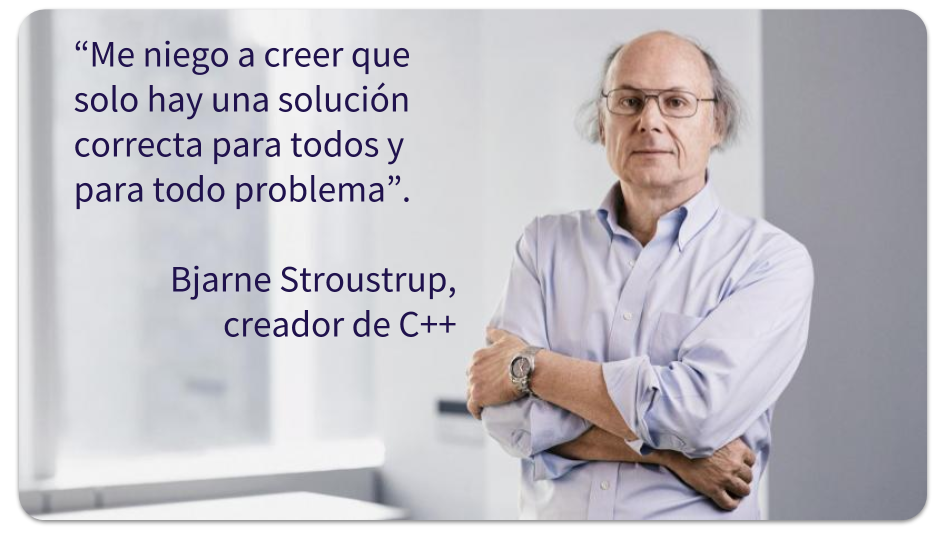
\includegraphics[width=1.0\textwidth]{CppIntro}
        \end{figure}


        % =========================================================
        % ==========          VENTAJAS DE C++        ==============
        % =========================================================
        \clearpage
        \section{Grandes ventajas de \Cpp}

            Hay muchas razones por las cuales \Cpp es uno de los lenguajes más usados en
            la modernidad en la programación competitiva (si no es que el más).

            Puedes escuchar un video muy bonito para mi sobre porque elegir este lenguaje:

            \Link{https://www.youtube.com/watch?v=JBjjnqG0BP8}{Bjarne Stroustrup: Why I Created \Cpp}

            \begin{figure}[h]
                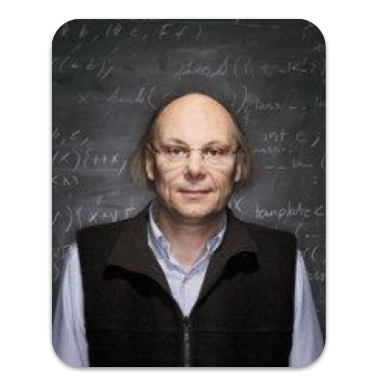
\includegraphics[width=0.35\textwidth]{BjarneBebe}
                \caption{\footnotesize{Este es el creador del lenguaje (reto: decir su nombre en voz alta) Bjarne Stroustrup}}
            \end{figure}


            Las principales razones por \Cpp sin un orden en particular son:
            \begin{itemize}
                \item \textbf{Te da abstracciones sin costo extra.}
                
                    O como lo diría su creador te da el poder de usar abstracciones de alto nivel pero estando muy cerca del hardware,
                    o como lo diría en inglés: 

                    \begin{Indentation}[1.2em]
                    \Quote{
                        C++ has the zero-overhead principle: \texttt{what you don’t use, you don’t pay for}, that is,
                        with every new feature added to the language, you get at least as good performance as
                        if that feature will not be included.
                        
                        Also there are the principle:
                        \texttt{What you do use cost either only as much as what you’d implement yourself, or it cost less}, 
                        meaning that a new feature can either mantain or improve the performance.
                    }
                    \end{Indentation}
                
                    Personalmente creo que esa es mayor ventaja que tiene sobre todos los demás, creo que
                    esa frase resume perfectamente todo el objetivo de \Cpp.

                    Lo que nos dice esto es que podremos representar grafos, matrices, operaciones, 
                    clases en general, algoritmos, etc... en nuestros programas con gran facilidad,
                    cosa que no podemos hacer fácilmente por ejemplo en lenguajes como C o la familia
                    de los ensambladores. 

                    \textit{
                    Y podrías decir, pero en Java o en Python podemos representar de una manera igual de fácil 
                    así que ... ¿porqué usar \Cpp?
                    }

                    Pues porque en todos los demás lenguajes estas pagando un costo (a veces muy grande de varios cientos 
                    o miles de veces) por poder representar ideas o conceptos abstractos en un programa, en \Cpp
                    esta prácticamente garantizado que usar una clase por ejemplo o que usar un arreglo que se auto
                    dimensiona no será más costoso que si lo hubieras hecho tu desde ensamblador.

                \item \textbf{Tienes a la biblioteca estandar, la gran std::* a tu lado}

                    Esta es otra gran ventaja, ya que siguiendo con la mentalidad de abstracciones sin costo extra tenemos
                    gracias a la gran libreria estándar un montón de cosas que no tenemos que hacer desde cero, desde
                    arreglos que cambian de tamaño, arreglos asociativos, pilas, colas, algoritmos de ordenamiento, 
                    de búsqueda, algoritmos para acumular, para hacer particiones o permutaciones, etc...

                    Así podemos dejar los algoritmos básicos al lenguaje y enfocarnos en las cosas que son de verdad interesantes.


                \item \textbf{Es compilado, el compilador es tu amigo}

                    Otra ventaja más, podemos siempre confiar en el compilador, en que si nuestro programa compila muy probablemente
                    está haciendo lo que debe hacer (cosa que no podemos esperar con python por ejemplo), el compilador es tu amigo,
                    te dira en donde te equivocaste, en donde puede que hayas querido decir otra cosa y muchas veces te dará
                    consejos, además, tras bambalinas está transformando tu código en algo que la computadora puede de verdad
                    entender y además usará toda la información que le diste para muchas veces incluso mejorar tu código en vez
                    de solo \Quote{traducirlo} y optimizarlo de maneras que me sorprenden personalmente.


                \item \textbf{Es prácticamente un \Quote{super set} de C}
                
                    Es decir, que
                    cualquier código válido de C es válido en \Cpp, esto es de gran ayuda pues
                    C es uno de los lenguajes más conocidos por lo que puede que la sintaxis de \Cpp sea
                    más fácil que entender la sintaxis de Haskell, por ejemplo. 
                    
                    Otra ventaja es que al estar basados
                    en C conserva muchas de las ventajas de C como su portabilidad, su velocidad de ejecución
                    y la capacidad de tener un gran control de todos los recursos del sistema (memoria y tiempo
                    de vida de un objecto, cough cough Java y su recolector de basura)

                \clearpage

                \item \textbf{Tienes un gran control de todos los recursos del sistema}
                
                    Esto es también es muy importante, pues nos dice que en \Cpp podemos controlar con gran lujo de detalle
                    los recursos del sistema, como por ejemplo la memoria.

                    \Cpp nos da el control de decidir por ejempo a que lugar va cada variable (heap o al stack), 
                    lo cual es esencial para un programa de alto rendimiento (y creeme que lo necesitaras).

                    \textbf{Es determinista.}

                    Es decir la limpieza de los objectos una vez que ya se acabaron de usar es solicitada cuanto tu quieres,
                    y no \textit{a ver cuando el recolector de basura decide hacerlo}.

                    Tenemos el control de decidir si queremos pasar las cosas por referencia o por valor, si deseamos mover
                    un objecto o si una referencia no podrá ser modificada.

                \item {Tienes \textit{value types} por defecto}.
                
                    Esta quiza sea algo rara de explicar si es que no sabes ningún lenguaje orientado a objectos, y si
                    no la entiendes no te preocupes. 

                    Lo que nos dice es que las variables en \Cpp son de tipo valor por defecto, es decir que
                    las podemos copiar, que nuestra variable de verdad almacenan la información que queremos \textbf{
                        y no una referencia (que apunta a quien sabe donde) de donde esta nuestra información
                    }.
                    Claro que aún puedes expresar la idea de las referencias, pero por defecto hablamos de variables
                    que almacenan valores.

            \end{itemize}


        % =========================================================
        % ==========             VS OTROS            ==============
        % =========================================================
        \clearpage
        \section{\Cpp vs otros lenguajes}

            % ============================================
            % ========          VS C        ==============
            % ============================================
            \subsection{vs C}

                El gran problema con C es que es un lenguaje muy pequeño en el sentido en que todo lo tienes que hacer tu,
                si quieres hacer un problema que involucra cosas medio complejas todas las estructuras las tienes que codear
                al momento, y en un deporte de tiempo, cada segundo cuenta, así que en resumén, lo que \Quote{mata} a C es la falta
                de algo parecido a la std de \Cpp.

                Aunque para problemas sencillos C también puede ser una opción, (pero ya que $\Cpp$ es casi casi
                un superset de C podrías entonces igualde fácil hacerlo en $\Cpp$).

            % ============================================
            % ==========       VS JAVA          ==========
            % ============================================
            \subsection{vs Java}

                Con toda honestidad hay un porcentaje de la comunidad de programación competitiva que usan Java, así que
                si que es una opción viable, sobretodo por su gran libreria estándar y también porque en C++ no hay algo parecido
                a \texttt{BigInteger} y \texttt{BigDecimal} y suelen ser muchos los problemas que lo requieran, así que si bien \Cpp
                podría ser tu lenguaje por defecto es importante que también conozcas lo básico de Java (O Kotlin si quieres ser feliz).

            % ============================================
            % ==========        VS PYTHON        =========
            % ============================================
            \subsection{vs Python}

                Python es un gran lenguaje pero tiene todas las de perder en programción competitiva pues
                a ser interpretado y debilmente tipado, sus programas acaban siendo muy lentos incluso usando el 
                algoritmo correcto, eso si, hay varias aplicaciones útiles de Python, como que todos los
                enteros tienen infinita precisión por defecto (aka \texttt{BigInteger} como en Java).

                Así que tampoco es una mala idea aprenderlo por si se necesita un día, pero definitivamente
                no es la mejor idea para ser tu lenguaje por defecto en programción competitiva.


        % =========================================================
        % ==========          CPP MODERNO            ==============
        % =========================================================
        \clearpage
        \section{ Una pincelada de \Cpp moderno}

            Incluso en términos solo de sintaxis te perdonaría si pensaras que \Cpp es un
            lenguaje terminado, algo que se hizo en los 90's y que seguimos escribiendo
            igual al día de hoy.

            Y no es así, \Cpp 11 / 14 / 17 / 20 son cosas muy diferentes, igual de flexibles
            y de rápidas que el clásico \Cpp 98 pero mucho mas seguro y limpio de escribir.

            Mira un ejemplo.

            \begin{lstlisting}[language=C++, gobble=16]
                //Old C++
                circle* p = new circle(42);
                vector<shape*> v = load_shapes();

                for (vector<shape*>:::iterator i = v.begin(): i != v.end(); ++i) {
                    if (*i && **i == *p)
                        cout << **i << "is a match" << endl;
                }

                // ...later, possible elsewhere

                for (vector<shape*>:::iterator i = v.begin(): i != v.end(); ++i) {
                    delete *i;
                }

                delete p;
            \end{lstlisting}

            Mientras que ahora podrías hacer algo como:
            \begin{lstlisting}[language=C++, gobble=16]
                //New badass C++
                auto p = make_shared<circle> (42);
                vector<shape*> v = load_shapes();

                for (auto& s : v) {
                    if (s && *s == *p)
                        cout << *s << "is a match" << endl;
                }
            \end{lstlisting}

            \clearpage

            Veamos otro ejemplo, imagina que alguien te da una secuencia de 
            puntos (flotantes por ejemplo) y te pide calcular su media.

            Veamos como sería hacerlo en Python así de volada:
            \begin{lstlisting}[language=python, gobble=16]
                def mean(seq):
                    n = 0.0
                    for x in seq:
                        n += x
                    return n / len(seq)
            \end{lstlisting}

            Y en \Cpp mira como sería:
            \begin{lstlisting}[language=C++, gobble=16]
                auto mean(const Sequence& seq) {
                    auto n {0.0};
                    for (auto x : seq)
                        n += x;
                    return n / seq.size();
                }
            \end{lstlisting}

            Que bonito, ¿no?
            \cite{ModernCppWhatYouNeedToKnow}


    % ===============================================================================
    % ===============             BASES DEL LENGUAJE          =======================
    % ===============================================================================
    \clearpage
    \chapter{Bases del Lenguaje}

        \begin{wrapfigure}{r}{0.15\textwidth}
            \centering
            
\includegraphics[width=0.15\textwidth]{Warning}
        \end{wrapfigure}

        \textbf{
            Recuerda que esta sección del texto NO es una introducción a la programación para
            alguien que nunca ha programado nada en su vida, sino solo para alguien que
            no sabe \Cpp. 
        }

        \textbf{
            Si este es tu caso entonces recomiendo que busques un documento, tutorial, libro, etc...
            diseñado para empezar a programar, porque en este texto voy a dar varias cosas por sentado
            que deberían ser muy obvias para alguien que ya haya aprendido a programar, en cualquier
            lenguaje.
        }

        \textbf{
            No te preocupes, te espero \texttt{<3}.
        }
        
        \textbf{
            Además si ya sabes \Cpp o no te interesa aprender toda la sintaxis e ir directo a cosas
            algo más relacionadas con la programación competitiva entonces puedes saltar hasta el
            siguiente capítulo.
        }

        % =========================================================
        % ========        VARIABLES SIMPLES          ==============
        % =========================================================
        \clearpage
        \section{Variables simples}

            En \Cpp (como en casi cualquier otro lenguaje) la idea obvia con la que podemos empezar
            es las variables.

            En \Cpp una variable es un fragmento de memoria (RAM) que almacena algun valor, 
            podemos tener variables que almacen lo que nosotros entenderemos como números enteros
            o que almacenen cadenas o que almacenen una secuencia de racionales etc...

            Bueno, \Cpp es un lenguaje de tipado estatico, es decir que todo momento el compilador
            (para poder transformar tu programa a algo que una computadora pueda entender) tiene
            que saber que tipo de dato almacena esa variable.

            Es decir, si yo quiero declarar una variable que almacene los días que llevo sin comer
            papas entonces podemos declararla de dos maneras en \Cpp.


            % ============================================
            % ====   DECLARACIONES E INICIALIZACION   ====
            % ============================================
            \subsection{Declaraciones e Inicialización}

                El primer paso para poder usar una variable será el de declararla, es decir
                aqui entre nos es decirle al compilador que te de un fragmento de RAM, que lo usaras
                para guardar un tipo de dato (numeros, matrices, texto, etc...) y que a este fragmento
                de RAM le pondras un nombre para poder referirte a el.

                Muy unido a esto decimos que estamos inicializando una variable cuando le damos
                un valor por primera vez a este espacio de RAM.

                Puedes declara variables en C++ de dos maneras:

                % ============================================
                % ======            SE DIRECTO          ======
                % ============================================
                \subsubsection{Se directo}

                    Algo como:
                    \begin{lstlisting}[language=C++, gobble=24]
                        int someNumber = 20;
                        string someText {"Hi baby"};
                        double myLoveForYou;
                    \end{lstlisting}

                    Es decir, la sintaxis es:
                    \begin{itemize}
                        \item Primero el tipo de dato, despues un espacio.
                        \item Despues el nombre que le quieres dar a la variable
                        \item Si quieres un valor inicial.
                    \end{itemize} 

                % ============================================
                % ======            SE SUTIL            ======
                % ============================================
                \subsubsection{auto: Se sútil}

                    Si es que es obvio que tipo de dato debería ser entonces puedes usar \texttt{auto}
                    que lo que nos dice es, compilador, yo se que eres un inteligente, anda, 
                    tu solito sabes de que tipo de dato es esta variable para que te lo repito yo.
                    
                    Y se hace hastante similar:
                    \begin{lstlisting}[language=C++, gobble=24]
                        auto someNumber = 20;   
                        auto someText {"Hi baby"};
                        auto myLoveForYou;          //This will fail
                    \end{lstlisting}

                    Nota que para que puedas usar auto el compilador tiene que saber que tipo
                    de dato va a guardar esa variable así que si no inicializas la variable 
                    el compilador se va a enojar contigo.

                De igual manera creo que te habras dado cuenta que podemos inicializar de dos maneras
                generalmente la primera es muy obvia y en casi todos los lenguajes existe, se llama
                una asignación, es decir, darle un valor a esa variable y se usa casi siempre en
                todos los Lenguaje el símbolo \texttt{=} o a veces incluso \texttt{<-}.

                Total, lo que pasa en \Cpp es que además de esa forma de inicializar weas tenemos
                una forma que si tiene un nombre especial.

                % ============================================
                % ======            SE SUTIL            ======
                % ============================================
                \subsubsection{Uniform Inizialization: Inicialización uniforme}

                    Y lo que nos da esto es una misma sintaxis, quiza esto sea un tema algo complejo
                    para unos y no te preocupes si no entiendes esto por completo por ahora.

                    Total, lo que pasa es que en \Cpp moderno existe la sintaxis 
                    \texttt{type wea \{something\}} donde lo que hacemos es poner entre estas cosas
                    \texttt{ \{ \} } el valor con el que queremos inicializar nuestra variable y dependiendo
                    de que sea nuestra variable puedes simplemente asignarla o llamar al constructor con estos
                    parámetro.

                    Total, es solo una forma mas bonita de hacer las cosas.

                    \begin{lstlisting}[language=C++, gobble=24]
                        auto someNumber {20};   
                        auto someText {"Hi baby"};
                        // this call a someClass constructor
                        someClass object {"some parameter", someNumber};
                    \end{lstlisting}


        % =========================================================
        % ======         TIPOS DE DATOS NUMERICOS          ========
        % =========================================================
        \clearpage
        \section{Tipos de datos numéricos}

            % ============================================
            % ======     INTEGERS: ENTEROS          ======
            % ============================================
            \subsection{Integers: Enteros}

                \Cpp (y C) maneja varios tamaños estándares de enteros, el más clásico
                es \texttt{int}, pero no es el único, los demás solo cambian en tamaño
                (y por los tanto los números que podemos almacenar)
                y estos son, de menor a mayor: \texttt{char, short, int, long y long long}.

                Así que con esto conocido, veamos las características más detalladamente de cada tipo:
                Pero si quieres un resumen, \Cpp garantiza que:
                \begin{lstlisting}[language=C++, gobble=20]
                    1 == sizeof(char) <= sizeof(short) <= sizeof(int) <= sizeof(long) <= sizeof(long long);
                \end{lstlisting}


                % ============================================
                % ==========        CHAR            ==========
                % ============================================
                \subsubsection{char}

                    A ver, técnicamente este tipo de dato como su nombre lo dice esta diseñado para almacenar
                    un carácter, lo que pasa es que en computación (no nos compliquemos la vida con UFT ahora)
                    un carácter como \texttt{'a'} ó \texttt{'p'} se representa internamente usando el código
                    ASCII (deberías buscar más de esto cuando tengas tiempo).
                    
                    Total, que en resumen este tipo de dato nació para almacenar un carácter de ASCII, 
                    por lo tanto es un tipo de datos numérico que va de 0 a 255.

                    No te preocupes si no entiendes las primeras líneas, pero si lo haces, muy bien por ti.
                    \begin{lstlisting}[language=C++, gobble=24]
                        auto character {'a'};                   // character is a char!
                        char number {23};                       // number is a char!
                        ('a' == 97) and ('z' == 122);           // true: ASCII is numbers
                        ('A' == 65) and ('Z' == 90);            // true: ASCII is numbers
                        ('A' + 1 == 'B') and ('Z' - 1 == 'Y');  // You can do arithmetic

                        auto size {"char is 1 byte"};
                        char minValue {-128};
                        char maxValue {127};
                    \end{lstlisting}


                % ============================================
                % ==========        INT            ===========
                % ============================================
                \clearpage
                \subsubsection{int}

                    Es el tipo de dato numérico estándar en \Cpp, así que si declaras un número
                    con \texttt{auto} entonces lo más probable es que sea \texttt{int}.

                    Ahora, pasa algo raro con este tipo de dato, que dependiendo de la máquina
                    en la que compiles entonces puede tener 2 o 4 bytes de tamaño (usa el que
                    sea más eficiente para el sistema), aun así, casi nunca compilaras en 
                    algún sistema que te diga que un \texttt{int} es de 2 bytes, así que para
                    este texto usaremos que \texttt{int} es de 4 bytes.
                    
                    \begin{lstlisting}[language=C++, gobble=24]
                        auto number {23};                           // number is an int!

                        auto size {"int is 4 bytes"};
                        int minValue {-2,147,483,648};
                        int maxValue {2,147,483,647};
                    \end{lstlisting}

                % ============================================
                % ==========        LONG           ===========
                % ============================================
                \subsubsection{long long}

                    Este no es un tipo de dato, per se, sino que es un modificador que le puedes aplicar
                    a \texttt{int} y con esto lo que logras es duplicar el tamaño de un int (suponiendo
                    que int tenga 4 bytes de tamaño, y creeme, seguramente es así).
                    
                    \begin{lstlisting}[language=C++, gobble=24]
                        int normalVariable {};                      // It takes 4 bytes     
                        long long int normalVariable {};            // It takes 8 bytes 
                        auto number {1,000,000,000,000,000,000}     // number is long long  

                        auto size {"long long int is 8 bytes"};
                        int minValue {-9,223,372,036,854,775,808};
                        int maxValue {9,223,372,036,854,775,807};
                    \end{lstlisting}


                % ============================================
                % ==========        UNSIGNED       ===========
                % ============================================
                \subsubsection{unsigned}

                    Lo que hace este modificador (exacto, esto tampoco es un tipo de dato)
                    es eliminar el signo de los tipos numéricos, es decir el entero más bajo que vas
                    a poder guardar va a ser el 0, pero con ello vas a lograr duplicar
                    el máximo entero que puedes almacenar y no aumentas para nada el espacio necesario :o
                    \begin{lstlisting}[language=C++, gobble=24]
                        char maxValueChar {127};                    
                        unsigned char maxValueIntUnsigned {255};
                        
                        int maxValueInt {2,147,483,647};                    
                        unsigned int maxValueIntUnsigned {4,294,967,295};
                        
                        long long maxValueLL {9,223,372,036,854,775,807};                    
                        unsigned long long maxValueLLUnsigned {18,446,744,073,709,551,615};
                    \end{lstlisting}


                % ============================================
                % ==========        UNSIGNED       ===========
                % ============================================
                \subsubsection{short}

                    Hace lo inverso que \texttt{long}, en vez que duplicar el tamaño lo parte a la mitad,
                    y ya, solo eso :v

                    \begin{lstlisting}[language=C++, gobble=24]
                        auto size {"short is 2 bytes"};
                        short int minValue {-32,768};
                        short int maxValue {32,767};
                    \end{lstlisting}
                
                % ============================================
                % ==========        SIZE_T         ===========
                % ============================================
                \subsubsection{std::size\_t}

                    Este es especial y muchas veces lo usaré como estándar de tipo numérico
                    y es que usamos muchas veces los enteros como índice de un contenedor.

                    Bien pues \texttt{size\_t} es un tipo de dato especial que nos da \Cpp
                    que nos asegura que será tan grande como necesitemos para usarlo como índice
                    de cualquier contenedor.

                    Nota que como lo usamos para índice, este tipo de dato no tiene signo.

                    Por ejemplo, \texttt{std::vector, std::string, std::array} y más lo usan
                    como índice.

                    \begin{lstlisting}[language=C++, gobble=24]
                        std::vector<int> someIntegers {1, 2, 3, 4, 20, 5};
                        std::size_t numberOfElements = {someIntegers.size()}; 
                    \end{lstlisting}
                    

            % ============================================
            % ====  FLOATING POINTS: PUNTO FLOTANTES  ====
            % ============================================
            \clearpage
            \subsection{Floating Points: Puntos Flotantes}

                A primera vista, los números de punto flotante parecen simples.
                Son solo enteros con puntos decimales, ¿verdad? 
                ¿Por qué no los usamos todo el tiempo, ya que pueden almacenar una mayor variedad de números?

                La respuesta es sencilla, no son precisos.

                \begin{figure}[h]
                    \centering
                    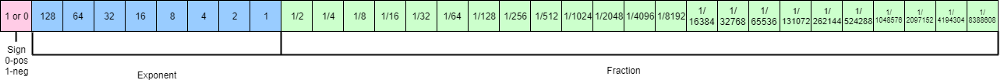
\includegraphics[width=0.9\textwidth]{IEEEFP}
                    \caption{\footnotesize{Representación del \texttt{float} en \Cpp}}
                \end{figure}

                Y ya, solo por eso, intenta poner en Python o en \Cpp si quieres esto 
                \texttt{(0.1 + 0.2) == 0.3} y verás que es falso, la razón es que los números de punto
                flotante tienen una cantidad límitada de dígitos de presición.

                Así que esta bien usarlos y todo, pero porfavor, hazlo con cuidado.

                Además así como \texttt{long long} era el doble que \texttt{int}, así
                \texttt{double} tiene el doble de presición (de ahí el nombre :v) que el clásico
                tipo de dato de punto flotante en \Cpp, \texttt{float}.

                \begin{lstlisting}[language=C++, gobble=20]
                    float almostPI {3.1};
                    double almostAlmostPI {3.14156};
                \end{lstlisting}
                

            % ============================================
            % =====  COMPLEX: NUMEROS COMPLEJOS     ======
            % ============================================
            \subsection{Complex: Números Complejos}

                Esta sección igual será corta, lo único que quiero decirte por si un día lo ocupas
                es que \Cpp tiene una clase que nos permite representar a los complejos.

                Nunca lo he ocupado de manera personal y no creo que sea el momento, en un texto introductorio
                de \Cpp, pero si un día lo necesitas, recuerda que \Cpp ya lo tiene integrado.

            
        % =========================================================
        % ==========             OPERADORES              ==========
        % =========================================================
        \clearpage
        \section{Operadores}

            % ============================================
            % =====      OPERADORES ARITMETICOS     ======
            % ============================================
            \subsection{Operadores Aritméticos}

                Sección corta, si sabes programar los has usado:

                \begin{itemize}
                    \item \texttt{+}: Suma
                    \item \texttt{-}: Resta
                    \item \texttt{*}: Multiplicación
                \end{itemize}

                Ahora los interesantes son los siguientes:

            % ============================================
            % =====         DIVISION ENTERA         ======
            % ============================================
            \subsection{División entera}

                Una cosa que a mucha gente le cuesta es la división y no porque
                sea una operación difícil sino porque en \Cpp dependiendo de los
                valores a los que se la apliquemos se comportara de manera correcta,
                si es que ambos valores son punto flotante entonces hara lo que esperas
                por ejemplo \texttt{1.0 / 2.0 = 0.5}, pero \texttt{1 / 2 != 0.5} porque
                si aplicas la división a dos enteros entonces hara la división y luego piso.

                Hay que tener cuidado con eso.

            % ============================================
            % =====              MODULO             ======
            % ============================================
            \subsection{Lo que hay que saber del módulo: \texttt{\%}}
            
                El módulo es pocas palabras es el residuo de la división.

                Es decir \texttt{a \% b} regresa el residuo de la división $\dfrac{a}{b}$
                si la has visto entonces verás que es la misma que en todos os lenguajes
                sino entonces mas vale que practiques con unos ejemplos, es todo cuestión
                de practica.

                % ============================================
                % =====              MODULO             ======
                % ============================================
                \subsubsection{La respuesta para los puristas}

                    Si eres matemático y quieres la definición formal podríamos pensar en:

                    \begin{MultiLineEquation*}{3}
                        a \% b = a - floor(a / b) * b
                    \end{MultiLineEquation*}

                    Otra forma de verlos es que nos regresa un número \texttt{k}
                    tal que $k \equiv a (\mod b)$

                % ============================================
                % =====              EJEMPLOS           ======
                % ============================================
                \subsubsection{Ejemplos}
                
                    \begin{itemize}
                        \item $7 \% 5 = 2$
                        \item $5 \% 7 = 5$
                        \item $3 \% 7 = 3$
                        \item $2 \% 7 = 2$
                        \item $1 \% 7 = 1$
                    \end{itemize}

                    Además, en general para lo único que lo usamos en general
                    es para saber si un número es par o impar, donde
                    si $n$ es par entonces \texttt{n \% 2 == 0} y si es impar
                    entonces \texttt{n \% 2 == 1}.

                    En general, si quieres saber si un número $n$ es multiplo de 
                    otro $k$ entonces hay que checar que $n \% k == 0$.


        % =========================================================
        % ==========        SENTENCIAS DE CONTROL        ==========
        % =========================================================
        \clearpage
        \section{Sentencias de Control}

            % ============================================
            % =======        CONDICIONALES         =======
            % ============================================
            \subsection{Condicionales}

                Sin una declaración de un condicional como la instrucción \texttt{if}, los programas
                se ejecutarán casi de la misma manera cada vez.
                
                Los condicionales permiten que se cambie el flujo del programa y con ello códigos
                más interesantes.

                \begin{lstlisting}[language=C++, gobble=20]
                    //Simpler form
                    if (condition) {
                        ...
                    }

                    //Simple form
                    if (condition) {
                        ...
                    }
                    else {
                        ...
                    }
                    
                    //Complete form
                    if (condition1) {
                        ...
                    }
                    else if (condition2) {
                        ...
                    }
                    else if (condition3) {
                        ...
                    }
                    else {
                        ...
                    }
                \end{lstlisting}


                % ============================================
                % =======        CONDICIONES           =======
                % ============================================
                \subsubsection{Condiciones}

                En \Cpp lo que puede ir dentro del \texttt{if (condition)} pueden ser dos cosas:
                \begin{itemize}
                    \item Se puede hacer \texttt{if (a = b)} en cuyo caso lo que comparará el 
                        \texttt{if} es el resultado de la asignación.
                    \item Una expresión que se pueda transformar a un \texttt{bool} y eso es la cosa
                        mas común.
                \end{itemize}

                % ============================================
                % =======        OPERADOR TERNARIO     =======
                % ============================================
                \subsubsection{Operador Ternario}

                En \Cpp tenemos el operador ternario, es bastante común porque nos deja expresar la misma
                idea que un \texttt{if} pero mucho mas corto, además es una expresión, es decir
                regresa un valor, esa es la más grande referencia.

                Y por lo tanto es muy útil cuando lo único que hacemos es darle un valor a una variable
                o algo relativamente sencillo.

                \begin{lstlisting}[language=C++, gobble=20]
                    // Using if else
                    if (language == "php") {
                        programmerFeelings = ":(";
                    }
                    else {
                        programmerFeelings = ":)";
                    }

                    // The same thing using ternary operator
                    happyProgrammer = language == "php" ? ":(" : ":)";
                \end{lstlisting}
                
        % =========================================================
        % ==========               CICLOS                ==========
        % =========================================================
        \clearpage
        \section{Ciclos}
            
            En \Cpp tenemos distintos tipos de ciclos, y si funcionan exactamente igual que
            en todos los demás lenguajes, tenemos:

            
            % ============================================
            % =======           WHILE              =======
            % ============================================
            \subsection{While}

                \begin{lstlisting}[language=C++, gobble=20]
                    while (condition) {
                        // statements
                    }
                \end{lstlisting}

                Donde condition es exactamente igual que lo que estaría dentro
                del if.

                % ============================================
                % =======          DO WHILE            =======
                % ============================================
                \subsubsection{Do while}

                    Existe también una variante que se llamada \texttt{do while} y que 
                    es bastante menos conocido que el clásico \texttt{while}, así que creo
                    que vale la pena hablar un poco de el.

                    \begin{lstlisting}[language=C++, gobble=24]
                        do {
                            // statements
                        }
                        while (condition);
                    \end{lstlisting}

                    En este ciclo primero ejecutamos las instrucciones que esten dentro del bloque
                    y luego es que checamos la condición y si es verdadera entonces volvemos 
                    ejecutar las instrucciones.

            % ============================================
            % =======           FOR                =======
            % ============================================
            \subsection{For}

                Igual que en cualquier otro lenguaje:
                \begin{lstlisting}[language=C++, gobble=20]
                    for (init expr; condition expr; step expr) {
                        // statements
                    }
                \end{lstlisting}

                Que como sabes si sabes programar es exactamente igual que:
                \begin{lstlisting}[language=C++, gobble=20]
                    init expr;
                    while (condition expr) {
                        // statements
                        step expr;
                    }
                \end{lstlisting}

                Ahora, hablemos del nuevo pequeño ciclo en el lenguaje:

            % ============================================
            % =======           FOR                =======
            % ============================================
            \subsection{\texttt{for (auto x : v)}}

                En \Cpp tenemos otra forma más moderna y muchos diran que mucho mas
                fácil de evitar bugs raros si lo único que haremos será movernos un 
                elemento a la vez a lo largo de un contenedor, y vamos a visitar cada
                elemento desde el inicio hasta el final del contendedor (no te preocupes, pronto
                hablaremos sobre contenedores) entonces puedes hacer un clásico:
                \begin{lstlisting}[language=C++, gobble=20]
                    for (type element : container) {
                        // statements
                    }
                \end{lstlisting}

                Por ejemplo:
                \begin{lstlisting}[language=C++, gobble=20]
                    vector<int> someNumbers {1, 2, 3, 4};

                    for (int i : someNumbers) {
                        cout << i << endl;
                    }
                \end{lstlisting}

                Y si, hablaremos sobre referencias y \texttt{auto\&\&} más a detalle pronto.

        % =========================================================
        % ====  REFERENCES AND VALUES:  APUNTADORES Y VALORES  ====
        % =========================================================
        \section{References and value types: Referencias o Valores}

            % ============================================
            % ====  VALUE TYPES: VARIABLES DE VALOR  =====
            % ============================================
            \subsection{Value types: Variables de valor}

            % ============================================
            % =====    POINTERS: APUNTADORES     =========
            % ============================================
            \subsection{Pointers: Apuntadores}

            % ============================================
            % =====    REFERENCIAS: REFERENCIAS     ======
            % ============================================
            \subsection{References: Referencias}
            

        % =========================================================
        % ==========             FUNCIONES               ==========
        % =========================================================
        \section{Funciones}

            Una función en \Cpp son practicamente iguales que en los demás lenguajes, pero
            en 

            % ============================================
            % ====            RECURSION         ==========
            % ============================================
            \subsection{Recursion}

            % ============================================
            % ====             LAMDAS           ==========
            % ============================================
            \subsection{Lamdas}

            % ============================================
            % ====             LAMDAS           ==========
            % ============================================
            \subsection{Lamdas}



    % ===============================================================================
    % ===============         CONTENEDORES STD              =========================
    % ===============================================================================
    \clearpage
    \chapter{Containers: Contenedores de la STD}

        % =========================================================
        % ==========             VECTOR                  ==========
        % =========================================================
        \section{std::vector}

            % ============================================
            % ===========       ARRAY      ===============
            % ============================================
            \subsection{std::array}

        
        % =========================================================
        % ==========             STRINGS                 ==========
        % =========================================================
        \section{std::string}


        % =========================================================
        % ==========             MAP                     ==========
        % =========================================================
        \section{std::map}

        % =========================================================
        % ==========             SET                     ==========
        % =========================================================
        \section{std::set}


    % ===============================================================================
    % ===================               CLASES          =============================
    % ===============================================================================
    \clearpage
    \chapter{Clases: OPP / POO}


    % ===============================================================================
    % ===================               SINTAXIS        =============================
    % ===============================================================================
    \clearpage
    \chapter{Cosas Avanzadas de \Cpp}

        % =========================================================
        % ==========            LIFETIME                 ==========
        % =========================================================
        \section{Lifetime: La mejor característica de \Cpp: \texttt{ \} } }     
        
            Se le pregunto a varios grandes programadores de \Cpp cual era su
            característica más importante y casi por unanimidad dijeron:

            \texttt{ \} }

            Y no, no estoy bromeando, este símbolo no es solo para decirle al compilador
            que se acaba de terminar el \texttt{scope} actual (es decir, que se acabo 
            la función o el bucle o la condicional o la clase, etc...) sino que es justo
            en este momento y solo en este momento cuando \Cpp limpia toda la basura.

            Por ejemplo dados estos códigos:
            \begin{lstlisting}[language=C++, gobble=16]
                int do_work() {
                    auto x = ...;
                }

                ...

                class shape {
                    container points;
                }
            \end{lstlisting}

            Es justo cuando el compilador ve \texttt{ \} } que se da la orden de limpiar,
            en ese momento es cuando se destruye la variable x o cuando destruyes a un objecto
            de tipo shape automaticamente se destruye el contenedor de puntos.
            
            En otras palabras porque las reglas de \Cpp sobre el \texttt{scope} de las variables
            y objectos te da una manera determinista y segura de finalizar weas.

            Es una forma automática y segura de liberar recursos cuando ya no los estoy usando.

            En otras palabras, la vida o \texttt{lifetime} de un objecto esta atada a su \texttt{scope}.
            Y como me gusta decirlo:
            \textbf{
                Todo el \Cpp es la responsabilidad de alguien
            }

            O en inglés:
            \textbf{
                Everything is owned by someone
            }

            \cite{ModernCppWhatYouNeedToKnow}

        % =========================================================
        % ==========           MOVE SEMANTICS            ==========
        % =========================================================
        \clearpage
        \section{Move Semantics: Semanticas de Movimiento}     
        
            En los viejos tiempo de \Cpp (y una de las razones por las que mucha gente cree que 
            el lenguaje es muy complejo) es porque la gente se preguntaba lo siguiente:

            \textit{Si tu me dijiste que \Cpp por defecto manera que sus variables son valores
            entonces tendrás que hacer un monton de cosas para evitar andar creando objectos (
                que a veces pueden ser enorme como una colección por ejemplo
            ) temporales y luego copiando toda su información, eso suena a algo muy costoso}

            Y debido a eso \Cpp 11 introdujo algo que se conoce como move semantics
            y esto es la idea de que si tienes una cosa muy compleja o muy enorme y tu la mueves
            (como por ejemplo los valores que te regresa una función) entonces \Cpp no simplemente 
            la copia toda completa sino que toma ownership o responsabilidad de sus entrañas
            (generalmente asignando un par de punteros) y deja ir al otro (ahora vacío) objecto listo para
            desaparecer.

            \cite{ModernCppWhatYouNeedToKnow}

        % =========================================================
        % ==========         VERDADEROS ARRAYS           ==========
        % =========================================================
        \clearpage
        \section{Si quieres un programa rápido: Verdaderos arrays}  
        
        % =========================================================
        % ==========         RANGE FOR STRANGE           ==========
        % =========================================================
        \clearpage
        \section{ \texttt{for (auto x : v)} vs \texttt{for (auto\& x : v)} vs \texttt{for (auto\&\& x : v)} }  
            




% //////////////////////////////////////////////////////////////////////////////////////////////////////////
% ///////////////////          TERMINOS DE CIENCIAS DE LA COMPUTACION              /////////////////////////
% //////////////////////////////////////////////////////////////////////////////////////////////////////////
\part{Ideas de las Ciencias de la Computación}
    

    % ===============================================================================
    % ==============                COMPLEJIDAD                       ===============
    % ===============================================================================
    \clearpage
    \chapter{La Complejidad}

        % =========================================================
        % ==========       COTAS Y NOTACIONES       ===============
        % =========================================================
        \section{Cotas y Notaciones}

            % ============================================
            % ====         REFERENCIAS          ==========
            % ============================================
            \subsection{Big O Notation: Notación de O grande}



    % ===============================================================================
    % ==============            OPTIMIZACION          ===============================
    % ===============================================================================
    \clearpage
    \chapter{Optimización}

        % =========================================================
        % ==========         OPTIMIZACION           ===============
        % =========================================================
        \section{Límites de Tiempo de Ejecución}

        % =========================================================
        % ==========         OPTIMIZACION           ===============
        % =========================================================
        \section{Límites de Memoria}



    % ===============================================================================
    % ==================         PROBLEMAS NP         ===============================
    % ===============================================================================
    \clearpage
    \chapter{Problemas NP}


% //////////////////////////////////////////////////////////////////////////////////////////////////////////
% ///////////////////                   ESTRUCTURAS DE DATOS                       /////////////////////////
% //////////////////////////////////////////////////////////////////////////////////////////////////////////
\part{Estructuras de Datos}

    % ===============================================================================
    % ================              ARRAYS            ===============================
    % ===============================================================================
    \clearpage
    \chapter{Arrays}

    % ===============================================================================
    % =============           STACKS LIFO: PILAS                      ===============
    % ===============================================================================
    \clearpage
    \chapter{Stacks LIFO: Pilas}

    % ===============================================================================
    % =============           QUEUE FIFO: COLAS                       ===============
    % ===============================================================================
    \clearpage
    \chapter{Queue FIFO: Colas}

    % ===============================================================================
    % ===========         LINKED LIST: LISTAS ENLAZADAS               ===============
    % ===============================================================================
    \clearpage
    \chapter{Linked Lists: Listas Enlazadas}


    % ===============================================================================
    % ==========             BINARY TREES: ARBOLES BINARIOS           ===============
    % ===============================================================================
    \clearpage
    \chapter{Binary Trees: Arboles Binarios}

        % =========================================================
        % =========      ARBOLES DE BUSQUEDA        ===============
        % =========================================================
        \section{BTS: Arboles de Búsqueda}

        % =========================================================
        % =========      ARBOLES AUTOBALANCEABLES       ===========
        % =========================================================
        \section{AVL - RedBlackTree: Arboles Autobalanceables}

        % =========================================================
        % =========                 TRIE                ===========
        % =========================================================
        \section{Trie}

    % ===============================================================================
    % =======================             HEAP         ==============================
    % ===============================================================================
    \clearpage
    \chapter{Heaps}


    % ===============================================================================
    % ==================           HASH TABLES         ==============================
    % ===============================================================================
    \clearpage
    \chapter{Hash Tables}


% //////////////////////////////////////////////////////////////////////////////////////////////////////////
% ///////////////////                   ALGORITMOS GENERALES                       /////////////////////////
% //////////////////////////////////////////////////////////////////////////////////////////////////////////
\part{Algoritmos Generales}
    
    % ===============================================================================
    % ================       SEARCH: BUSQUEDAS         ==============================
    % ===============================================================================
    \clearpage
    \chapter{Search: Búsquedas}

        % =========================================================
        % ======    LINEAR SEARCH: BUSQUEDA LINEAL           ======
        % =========================================================
        \section{Linear Search: Búsqueda Lineal}

        % =========================================================
        % ======    BINARY SEARCH: BUSQUEDA BINARIA          ======
        % =========================================================
        \section{Binary Search: Búsqueda Binaria}

        % =========================================================
        % ======    TERNARY SEARCH: BUSQUEDA TERNARIA        ======
        % =========================================================
        \section{Ternary Search: Búsqueda Ternaria}

        % =========================================================
        % =======              UPPER BOUND          ===============
        % =========================================================
        \section{Upper Bound}

        % =========================================================
        % =======              LOWER BOUND          ===============
        % =========================================================
        \section{Lower Bound}



    % ===============================================================================
    % ================       SORTING: ORDENAMIENTO     ==============================
    % ===============================================================================
    \clearpage
    \chapter{Sorting: Ordenamiento por Comparaciones}

        % =========================================================
        % ==========            BUBBLE SORT         ===============
        % =========================================================
        \section{Bubble Sort}

        % =========================================================
        % ==========            SELECTION SORT      ===============
        % =========================================================
        \section{Selection Sort}

        % =========================================================
        % ==========            MERGE SORT         ===============
        % =========================================================
        \section{Merge Sort}

        % =========================================================
        % ==========            QUICK SORT          ===============
        % =========================================================
        \section{Quick Sort}



    % ===============================================================================
    % ================       SORTING: ORDENAMIENTO     ==============================
    % ===============================================================================
    \clearpage
    \chapter{Sorting: Ordenamiento NO por Comparaciones}
        
        % =========================================================
        % ==========            BUCKET SORT         ===============
        % =========================================================
        \section{Bucket Sort}



% //////////////////////////////////////////////////////////////////////////////////////////////////////////
% ///////////////////                   MATEMATICAS                                /////////////////////////
% //////////////////////////////////////////////////////////////////////////////////////////////////////////
\part{Programación es solo matemáticas aplicadas}

    % ===============================================================================
    % ==========                   BINARY: BINARIO                    ===============
    % ===============================================================================
    \clearpage
    \chapter{Binary: Explotando el Binario}

        % =========================================================
        % =======                  BITS             ===============
        % =========================================================
        \section{Bits}

            % ============================================
            % =======        MANEJO DE BITS      =========
            % ============================================
            \subsection{Manejo de Bits}

            % ============================================
            % =======        MANEJO DE BITS       ========
            % ============================================
            \subsection{Operaciones con Bits}

        % =========================================================
        % ======      CONVERSIONES ENTRE SISTEMAS         =========
        % =========================================================
        \section{Conversiones entre Sistemas}

        % =========================================================
        % =======        EXPONENCIACION BINARIA        ============
        % =========================================================
        \section{Binary Exponentiation: Exponenciacion Binaria}

        % =========================================================
        % =======        MULTIPLICACION BINARIA        ============
        % =========================================================
        \section{Binary Multiplication: Multiplicación Binaria}



    % ===============================================================================
    % ==========                    ENCONTRAR RAÍCES                    =============
    % ===============================================================================
    \clearpage
    \chapter{Roots: Encontrar Raíces de ecuaciones}

        % =========================================================
        % =======        NEWTON RANPHSON            ===============
        % =========================================================
        \section{Newton - Ranphson}


    
    % ===============================================================================
    % ==========                 TEORIA DE NUMEROS                      =============
    % ===============================================================================
    \clearpage
    \chapter{Teoría de Números}

        % =========================================================
        % =======        DIVISIBILIDAD              ===============
        % =========================================================
        \section{Divisibilidad}

            % ============================================
            % =====       EUCLIDES               =========
            % ============================================
            \subsection{Euclides}

        % =========================================================
        % =======        MODULOS                    ===============
        % =========================================================
        \section{Modulos}

        % =========================================================
        % =======        FIBONACCI                  ===============
        % =========================================================
        \section{Fibonacci}

        % =========================================================
        % =======        FIBONACCI                  ===============
        % =========================================================
        \section{Números de Catalán}

        % =========================================================
        % =======               PRIMOS              ===============
        % =========================================================
        \section{Primos y Factores}

            % ============================================
            % ======      CRIBA DE ERATOSTENES      ======
            % ============================================
            \subsection{Eratosthenes Sieve: Criba de Eratóstenes}

            % ============================================
            % ====          FACTORIZACION          =======
            % ============================================
            \subsection{Prime Factorization: Factorización}

            % ============================================
            % ====             DIVISORES           =======
            % ============================================
            \subsection{Divisores}

            % ============================================
            % ====        PHI DE EULER             =======
            % ============================================
            \subsection{Euler Totient: La Phi de Euler}


    % ===============================================================================
    % ==========                    PROBABILIDAD                      ===============
    % ===============================================================================
    \clearpage
    \chapter{Probabilidad}

        % =========================================================
        % =======        INCLUSION EXCLUSION        ===============
        % =========================================================
        \section{Inclusión Exclusión}

  
    % ===============================================================================
    % ==================                  GEOMETRIA                ==================
    % ===============================================================================
    \clearpage
    \chapter{Geometría}


% //////////////////////////////////////////////////////////////////////////////////////////////////////////
% ///////////////////                   TECNICAS DE SOLUCION                       /////////////////////////
% //////////////////////////////////////////////////////////////////////////////////////////////////////////
\part{Técnicas de Solución}

    % ===============================================================================
    % ==========                        AD-HOC                        ===============
    % ===============================================================================
    \clearpage
    \chapter{Ad-Hoc}

    
    % ===============================================================================
    % ===============            RECURSIVIDAD Y BACKTRAKING           ===============
    % ===============================================================================
    \clearpage
    \chapter{Recursividad y BackTracking}

    % ===============================================================================
    % ==========                DIVIDE Y VENCERAS                     ===============
    % ===============================================================================
    \clearpage
    \chapter{Divide and Conquer: Divide y Vencerás}


    % ===============================================================================
    % ========================            GREEDY             ========================
    % ===============================================================================
    \clearpage
    \chapter{Greedy}

    % ===============================================================================
    % =========            PROGRAMACION DINAMICA             ========================
    % ===============================================================================
    \clearpage
    \chapter{Programación Dinámica}


% //////////////////////////////////////////////////////////////////////////////////////////////////////////
% ///////////////////                   GRAFOS Y FLUJOS                            /////////////////////////
% //////////////////////////////////////////////////////////////////////////////////////////////////////////
\part{Grafos y Flujos}

    % ===============================================================================
    % ==========                         GRAFOS                       ===============
    % ===============================================================================
    \chapter{Grafos y Gráficas}    

        % =========================================================
        % ==========        REPRESENTACIONES        ===============
        % =========================================================
        \section{Representaciones}

        % =========================================================
        % ==========        BREADTH FIRST SEARCH       ============
        % =========================================================
        \section{BFS: Breadth-first Search}


        % =========================================================
        % ==========        DEPTH FIRST SEARCH         ============
        % =========================================================
        \section{DFS: Depth-first Search}

        % =========================================================
        % ==========        REPRESENTACIONES        ===============
        % =========================================================
        \section{Dijsktra: Camino más cercano}



% ===============================================
% ========        BIBLIO      ===================
% ===============================================
\begin{thebibliography}{10}

    \bibitem{CP3} 
        Competitive Programming 3,
        \textit{Halim and Halim, 2013}. 


        \bibitem{ModernCppWhatYouNeedToKnow} 
        Build Conference: Modern C++ what you need to know
        \textit{Herb Sutter, 2014}. 

\end{thebibliography}


\end{document}